\chapter{Results and Discussion}
\label{cha:result}
In this section we apply techniques introduced in \cref{cha:methodology} to test our new methods for nefarious router classification. We present results of nefarious router classification under assumption sets one, two, and three in \cref{ssec:Ras1,ssec:Ras2,ssec:Ras3} respectively. We summarise our findings and comparisons between classifier in \cref{ssec:Rnefidsummary}. Comparisons focus on classifiers two and three as classifier one uses delay distribution not obtainable with network tomography. We then present results from testing of optimised probe path selection and probe allocation in \cref{sec:Rprobingoptimality}. Validation of model correctness with respect to assumptions regarding queue length stabilisation, noted as a requirement in previous work, is presented in Appendix A.

\section{Identifying Nefarious Behaviour}
\label{sec:Rnefarouterdetection}
For numerical analysis of classification under our proposed three assumption sets we consider the Nobel, Free, and CPLEX network topologies. This allows us to provide a robust analysis of analytical results using confusion matrices for each classification scenario. For each assumption set we discuss the classifiers performance under each scenario and provide generalised evaluations of each classifier, begin with assumption set one.

\subsection{Classifier One}
\label{ssec:Ras1}
Firstly we consider classification with a full delay distribution and baseline comparisons. Confusion matrices for nefarious node classification are shown in \cref{tab:ngercmatrix,tbl:frncecmatrix,tbl:nrwycmatrix}. Each classification was performed using a KS comparison against the true baseline values and a p-val cutoff of 0.0 to provide the strictly possible guarantee of significance.\par
\noindent
\begin{table}[H]
    \centering
    \aboverulesep = 0pt
    \belowrulesep = 0pt
    \begin{tabular}{l|cc}
        {\backslashbox{\textit{Actual}}{\textit{Predicted}}} & {Nefarious} & {Non-nefarious}\\
        \midrule
        {Nefarious}     & 1807  & 0     \\
        {Non-nefarious} & 37    & 3018  \\
    \end{tabular}
    \caption{Confusion matrix for classification under assumption set 1 in the Nobel topology.}
    \label{tab:ngercmatrix}
\end{table}
\noindent
\begin{table}[H]
    \centering
    \aboverulesep = 0pt
    \belowrulesep = 0pt
    \begin{tabular}{l|cc}
        {\backslashbox{\textit{Actual}}{\textit{Predicted}}} & {Nefarious} & {Non-nefarious}\\
        \midrule
        {Nefarious}     & 2781  & 101     \\
        {Non-nefarious} & 101    & 2658  \\
    \end{tabular}
    \caption{Confusion matrix for classification under assumption set 1 in the Free topology.}
    \label{tbl:frncecmatrix}
\end{table}
\noindent
\begin{table}[H]
    \centering
    \aboverulesep = 0pt
    \belowrulesep = 0pt
    \begin{tabular}{l|cc}
        {\backslashbox{\textit{Actual}}{\textit{Predicted}}} & {Nefarious} & {Non-nefarious}\\
        \midrule
        {Nefarious}     & 1905  & 46     \\
        {Non-nefarious} & 413   & 1896   \\
    \end{tabular}
    \caption{Confusion matrix for classification under assumption set 1 in the CPLEX topology.}
    \label{tbl:nrwycmatrix}
\end{table}
Classification in the Nobel topology has a sensitivity of 100\% across all evaluated sets of nefarious routers. With 37 false positives the classifier has a specificity of 99.99\%, giving an extremely precise and accurate nefarious node classification. For the Free and CPLEX topologies we observe marginally worse classification performance. The classifier has a sensitivity of 96.5\% and 97.64\% and a specificity of 96.34\% and 82.11\% for Free and CPLEX respectively. Given the efficacy of classification over all topologies we omit discussion under each scenario, as each would be near perfect, in favour of focusing on the general classification results and trends between topologies.\par
The most striking result is a sensitivity of 100\% in the Nobel topology, closely followed by the 99.9\% specificity in the same topology. We anticipate the extreme efficacy of this classification is due to the relatively small number of routers within the Nobel topology allowing us to obtain router identifiability using only 28 probe paths. The reduction in classifier performance as the size of the topology increases support this theory.\par
This trend is likely due to the number of probe paths required to achieve router identifiability in each topology. With fewer probe paths producing a robust average of metrics in each probe path. We would however expect the true sensitivity of the classifier to however be <100\% but the sample size needed to determine this would be prohibitively large.\par
In all topologies we observe the classifier having a higher sensitivity than specificity. This is likely due to the stochastic routing behaviour of the network routing packets away from nefarious routers which will have larger buffer queues. This would cause non-nefarious routers to receive more packets and subsequently a larger buffer queue appearing nefarious. Nefarious routers however - even when forwarded few packets - will still delay a proportion of these packet. These routers will therefore maintain a larger queue length, enabling their classification from packet delay metrics and minimising false negatives.\par

\subsection{Classifier Two}
\label{ssec:Ras2}
Next we consider classification with a baseline comparison and only packet delay summary statics available. ROC curves for classification in each topology are given in \cref{fig:RA2ROCcurves}. Note the performance of the classifier under each case is extrapolated from a corresponding point lying on the ROC curve.\par
For scenario one router classification in the Nobel, Free, and CPLEX topologies satisfied the sensitivity threshold of 0.9 with a false positive rate of 0.811, 0.838, and 0.919 respectively. Classification in the Nobel and Free topologies is superior to random classification of routers. However, with a sensitivity of > 0.763 the classification accuracy for the CPLEX network is worse than random. This is due to a sympathetic increase between non-nefarious router PDA (over baseline PDA) and nefarious router PDA. The sympathetic increase is caused by the link-state protocol routing packets around nefarious routers as their buffer queue's fill. This results in more packets being forwarded to non-nefarious routers over the baseline simulation, increasing the difference in PDA from the baseline simulation.\par
For scenario two the classifier reaches the 0.7 sensitivity threshold in the Nobel, Free, and CPLEX topologies with a false positive rate of 0.392, 0.426, and 0.669 respectively. For scenario three the 0.9 specificity threshold is satisfied with a false negative rate of 0.558, 0.682, and 0.864 for each topology respectively.\par
In both scenario two and three all classifier perform better than a random classification. However for scenario two classification in the CPLEX topology is notably worse than the Nobel and Free topologies, even when accounting for the increased number of routers. We anticipate this is caused by the same factors as in scenario one, likely increased noise in probe path measurements. In general however less stringent sensitivity requirements reduce the impact of noise on classification.\par
With scenario three's requirements on specificity the reduction in classifier accuracy is proportional to the number of routers in each topology. Additionally across all topologies the classifier performs the best relative to a random classification in sensitivity and specificity ranges of [0.2, 0.76] and [0.24, 0.83] respectively. Classification under assumption case two is therefore better suited to use cases with a higher tolerance for false negatives.\par
\noindent
\begin{figure}[H]
    \centering
    \begin{subfigure}{0.475\textwidth}
        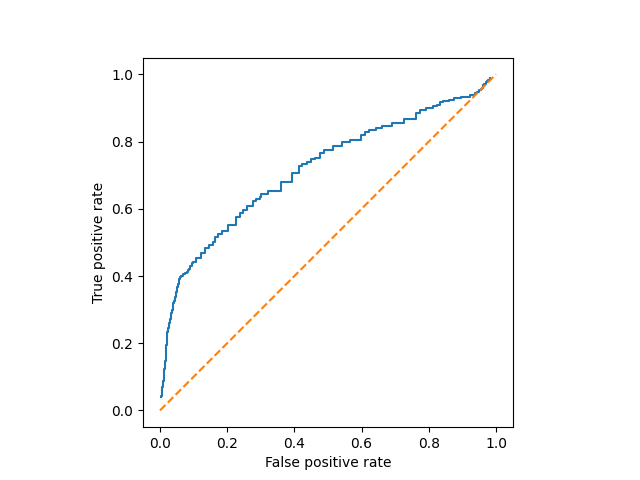
\includegraphics[width=\textwidth]{figs/results/nobel-germany_case2_roc.png}
        \caption{Nobel Topology.}
    \end{subfigure}
    \begin{subfigure}{0.475\textwidth}
        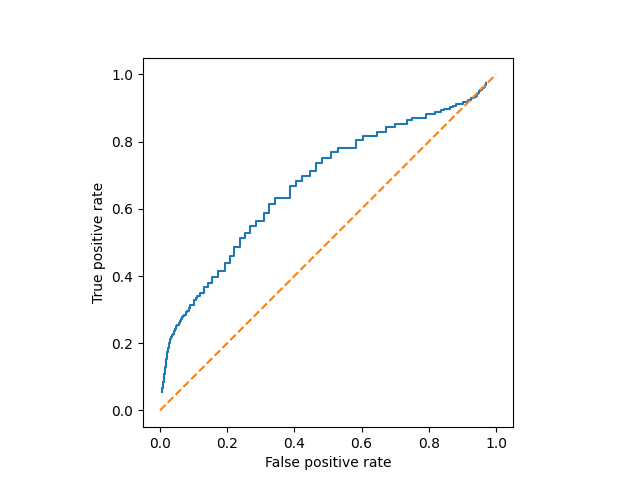
\includegraphics[width=\textwidth]{figs/results/france_case2_roc.png}
        \caption{Free Topology.}
    \end{subfigure}
    \begin{subfigure}{0.475\textwidth}
        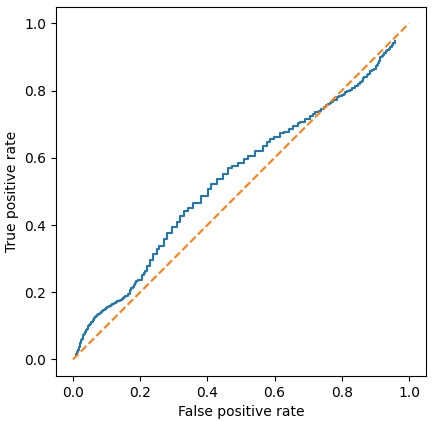
\includegraphics[width=\textwidth]{figs/results/norway_case2_roc.png}
        \caption{CPLEX Topology.}
    \end{subfigure}
    \caption{ROC curves for classification under assumption set 2.}
    \label{fig:RA2ROCcurves}
\end{figure}

\subsection{Classifier Three}
\label{ssec:Ras3}
\noindent
\begin{figure}
    \centering
    \begin{subfigure}{0.475\textwidth}
        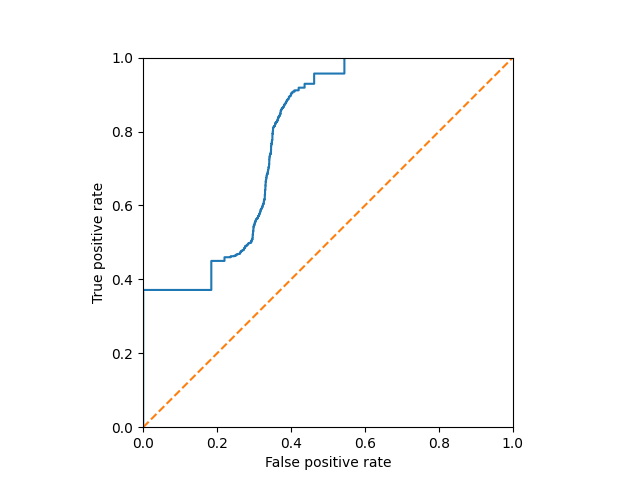
\includegraphics[width=\textwidth]{figs/results/nobel-germany_case3_roc.png}
        \caption{Nobel Topology.}
    \end{subfigure}
    \begin{subfigure}{0.475\textwidth}
        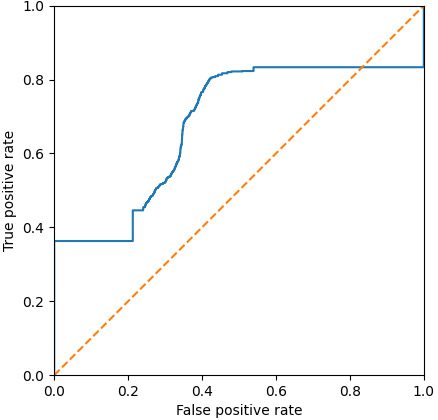
\includegraphics[width=\textwidth]{figs/results/france_case3_roc.png}
        \caption{Free Topology.}
    \end{subfigure}
    \begin{subfigure}{0.475\textwidth}
        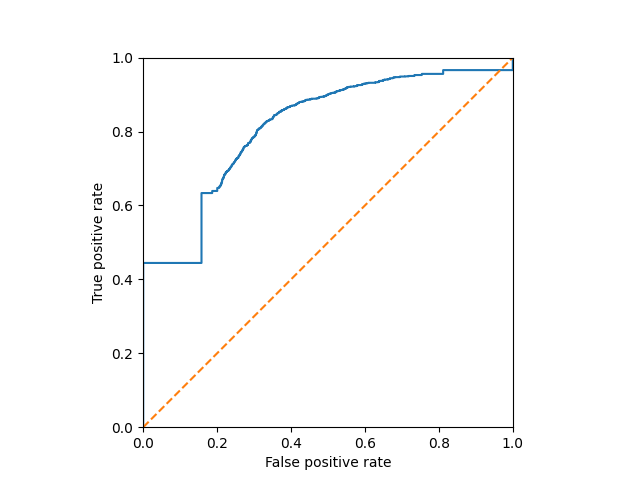
\includegraphics[width=\textwidth]{figs/results/norway_case3_roc.png}
        \caption{CPLEX Topology.}
    \end{subfigure}
    \caption{ROC curves for classification under assumption set 3.}
    \label{fig:RA3ROCcurves}
\end{figure}
Finally we use only packet delay summary statics for classification. ROC curves for classification in each topology are given in \cref{fig:RA3ROCcurves}. We evaluate the classifiers performance for each scenario below.\par
For scenario one classification of the Nobel and CPLEX topologies results in a false positive rate of 0.4 and 0.5 respectively. For the Free topology the classifier is only able to attain a sensitivity of 0.9 with a false negative rate of 1.0 (classify all routers as nefarious). Excluding this case, PDA is not sufficient to classify routers with a sensitivity greater than 0.83 in the Free topology.\par
This is due to the topology containing a node with a degree of 10 (Paris). The Paris node experiences more than twice as much traffic as the average node of degree 3 and thus has a near or completely full queue buffer regardless of nefarious behaviour. This is compounded by 15 of the 37 probe paths including Paris, resulting in a disproportionate number of probe packets traversing the router. Therefore when using a PDA threshold of buffer queue length $-\epsilon$ for classification the Paris node is always classified as nefarious. A similar limitation exists in the CPLEX topology where due to the same factors where a maximum sensitivity of 0.966 can be achieved.\par
Conversely, the classifier performs extremely well on the Nobel topology achieving a true positive rate of 1.0 with a false positive rate of 0.544. Although both Nobel and CPLEX have a maximum node degree of 6, in the Nobel network only 12 probe paths traverse the maximally connected router compared to 21 in CPLEX. Therefore in the CPLEX network, unlike the Free network, the maximally connected router's buffer queue receives disproportionately more probe packets. This results in the router being classified as nefarious regardless of its delaying behaviour in the majority of test trials.\par
For scenario two classification of the Nobel, Free, and CPLEX topologies results in a false positive rate of 0.339, 0.363, and 0.235 respectively. These rates are a strict improvement over classification under assumption case two. This improvement is due to the increased queue length of nefarious routers due to their delaying causing a tendency for traffic to be directed through non-nefarious routers. This increases the queue length of these non-nefarious routers, resulting in more cases of incorrectly classifying a router as nefarious.\par
For scenario three classification of each topology results in a false negative rate of 0.629 for the Nobel and Free topologies and 0.556 for CPLEX. However, for each case in \cref{fig:RA3ROCcurves} no PDA thresholds enable a classification with a false positive rate < 0.2. This is due to an overlap in PDA values between weakly connected nefarious router and strongly connected non-nefarious routers. The amount of traffic arriving at strongly connected non-nefarious routers fills their buffer queue at a rate similar to a less connected nefarious router. Therefore a PDA threshold sufficient to identify any weakly connected routers also causes false positives.\par

\subsection{Summary of Comparisons}
\label{ssec:Rnefidsummary}
In this section we have analysed three nefarious routers classifiers with three real-world use cases for a fair comparison of performance. Classifier one was found to have the best performance in each use case. This classifier achieved a near perfect accuracy across all investigated topologies. However, as this underlying distribution can not be obtained via network tomography we focused our comparison on the second and third classifiers.\par
Classifier two was found to perform better than a random classification in all cases other than in the CPLEX topology with a sensitivity > 0.763. This was caused by a sympathetic increase between non-nefarious router PDA (over baseline PDA) and nefarious router PDA due to stochastic traffic routing. This classifier performed optimally for specificity requirements between 0.24 and 0.83 across all topologies.\par
Classifier three achieved greater accuracy than classifier two for sensitivity and specificity requirements of [0.2, 0.83] and [0.46, 0.75] respectively. This was due to absence of baseline comparisons causing sympathetic increases between routers to not impact classification. However, classifier two performed very poorly for sensitivities below 0.2 and above 0.8. This was due to an overlap in PDA metrics between strongly connected non-nefarious and weakly connected nefarious.

\section{Optimisation Impacts}
\label{sec:Rprobingoptimality}
In this section we apply optimization techniques for selection of probe paths between monitor nodes and allocation of probe packets between paths. Inference made under optimized conditions are compared and contrasted to original measures to quantify impact of optimizations, computational costs involved in optimization techniques are weighed against changes in accuracy to assess the practicality of implement these improvements in tomographic monitoring schemes.

\subsection{Path Selection}
\label{ssec:Rpathselection}
\noindent
\begin{figure}
    \centering
    \begin{subfigure}{0.475\textwidth}
        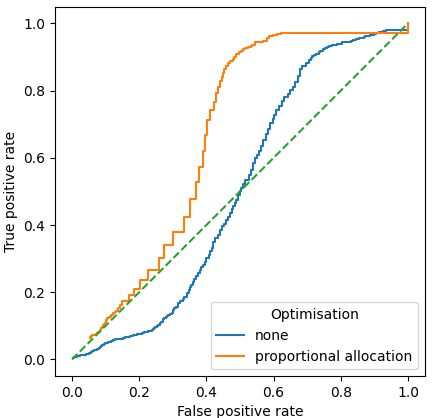
\includegraphics[width=\textwidth]{figs/results/nobel-germany_ac2_opt.png}
        \caption{Nobel Topology.}
    \end{subfigure}
    \begin{subfigure}{0.475\textwidth}
        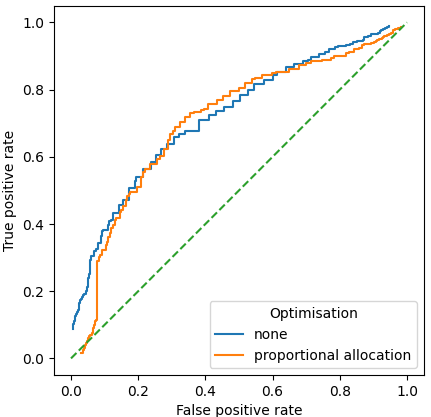
\includegraphics[width=\textwidth]{figs/results/france_ac2_opt.png}
        \caption{Free Topology.}
    \end{subfigure}
    \begin{subfigure}{0.475\textwidth}
        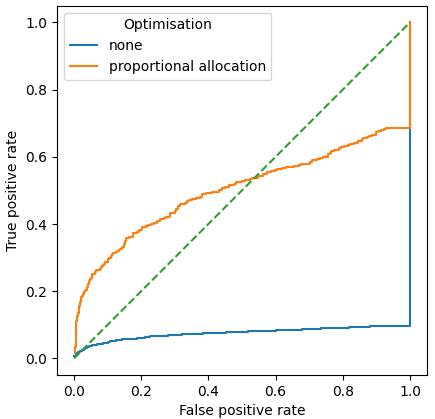
\includegraphics[width=\textwidth]{figs/results/norway_ac2_opt.png}
        \caption{CPLEX Topology.}
    \end{subfigure}
    \caption{ROC curves for optimised classification under assumption set 2.}
    \label{fig:RprobeoptA2ROCcurves}
\end{figure}

\noindent
\begin{figure}
    \centering
    \begin{subfigure}{0.475\textwidth}
        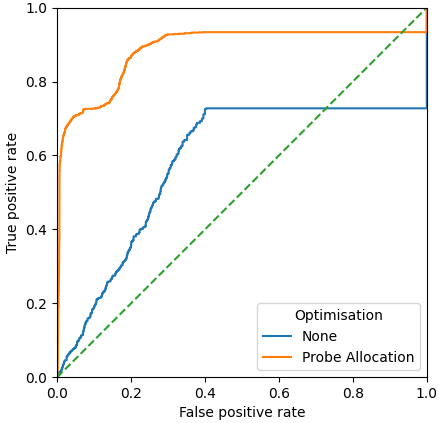
\includegraphics[width=\textwidth]{figs/results/nobel-germany_ac3_opt.png}
        \caption{Nobel Topology.}
    \end{subfigure}
    \begin{subfigure}{0.475\textwidth}
        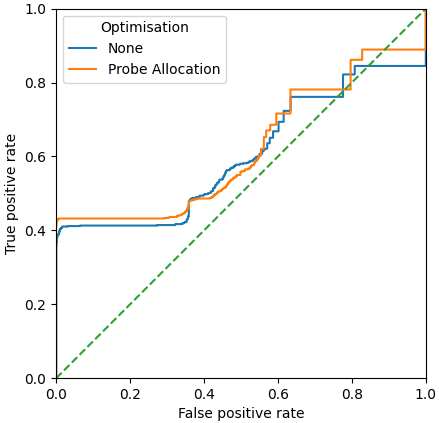
\includegraphics[width=\textwidth]{figs/results/france_ac3_opt.png}
        \caption{Free Topology.}
    \end{subfigure}
    \begin{subfigure}{0.475\textwidth}
        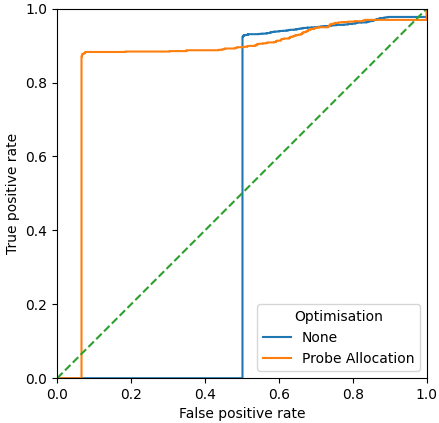
\includegraphics[width=\textwidth]{figs/results/norway_ac3_opt.png}
        \caption{CPLEX Topology.}
    \end{subfigure}
    \caption{ROC curves for optimised classification under assumption set 3.}
    \label{fig:RprobeoptA3ROCcurves}
\end{figure}

\subsection{Probe Allocation}
\label{ssec:Rprobeallocation}

\section{Summary}
